\documentclass[tikz,border=6pt]{standalone}
\usepackage{amsmath}
\usepackage{xcolor}
\usetikzlibrary{arrows.meta,positioning}

\definecolor{blockblue}{HTML}{4A90D9}
\definecolor{linegray}{HTML}{333333}

\begin{document}
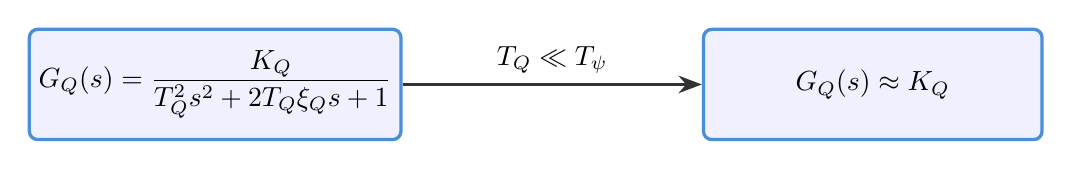
\begin{tikzpicture}[
  >=Stealth,
  line width=1.2pt,
  block/.style={draw=blockblue, rounded corners=3pt, minimum width=4.3cm, minimum height=1.4cm, align=center, fill=blue!6},
  flow/.style={->, draw=linegray, line width=1.2pt}
]
  \node[block] (full) at (0,0) {$G_Q(s)=\dfrac{K_Q}{T_Q^2s^2 + 2T_Q\xi_Q s + 1}$};
  \node[block, right=3.8cm of full] (approx) {$G_Q(s)\approx K_Q$};
  \draw[flow] (full) -- node[above] {$T_Q \ll T_\psi$} (approx);
\end{tikzpicture}
\end{document}
